% GENERATED by scripts/make_sim_figures.py from simulation
% campaign 20260831_001736+20260831_002055. Do not edit: re-run the campaign instead.
% the per-joint clamp against its own step size
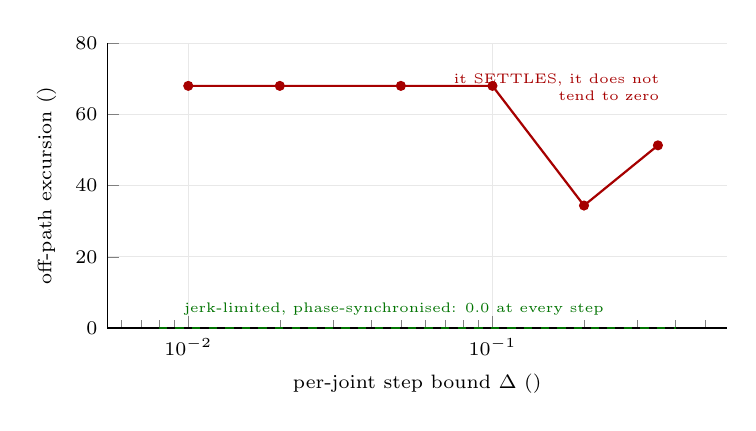
\begin{tikzpicture}
\begin{axis}[
    width=0.78\linewidth, height=52mm,
    xmode=log, log basis x=10,
    xlabel={per-joint step bound $\Delta$ (\si{\radian})},
    ylabel={off-path excursion (\si{\milli\metre})},
    xlabel style={font=\scriptsize}, ylabel style={font=\scriptsize},
    tick label style={font=\scriptsize},
    axis lines*=left, grid=major, grid style={gray!18},
    ymin=0, ymax=80,
]
\addplot[red!65!black, thick, mark=*, mark size=1.4pt] coordinates {(0.35,51.3) (0.20,34.4) (0.10,68.0) (0.05,68.0) (0.02,68.0) (0.01,68.0)};
\addplot[green!45!black, thick, dashed] coordinates {(0.008,0)(0.4,0)};
\node[font=\tiny, green!45!black, anchor=south west]
  at (axis cs:0.009,1) {jerk-limited, phase-synchronised: \SI{0.0}{\milli\metre} at every step};
\node[font=\tiny, red!65!black, anchor=north east, align=right]
  at (axis cs:0.38,74) {it SETTLES, it does not\\tend to zero};
\end{axis}
\end{tikzpicture}
